\documentclass[a4paper]{article}

\usepackage{polski}
\usepackage[utf8]{inputenc}
\usepackage[pdftex]{graphicx}
\usepackage{fancyhdr}
\usepackage{float}

\newcommand{\prog}{\texttt}

\linespread{1.15}
\pagestyle{fancy}
\fancyhf{}
\chead{Specyfikacja funkcjonalna}
\cfoot{Strona \thepage \ z \pageref{end}}

\title{Specyfikacja funkcjonalna\\Projekt \textit{Gra Galaxy Defender} w języku Java}
\author{Jakub Czajka (299239)\\Daniel Daczko (299241)}

\begin{document}

\maketitle
\tableofcontents
\thispagestyle{empty}

\section{Opis ogólny}

\subsection{Nazwa programu}
Jako nazwę programu przyjęliśmy wyrażenie \prog{Galaxy Defender}, które można przetłumaczyć z języka angielskiego jako \textit{Obrońca Galaktyk}. Jest to ścisłe nawiązanie do graficznego interfejsu naszej gry.

\subsection{Poruszany problem}
\textit{Galaxy Defender} jest grą typu multiplayer shooter. Wykorzystuje ona grafikę dwuwymiarową. Gra inspirowana jest dwoma klasycznymi tytułami:
\begin{itemize}
    \item \textit{Space Invaders}, z których czerpie sposób eliminacji wrogów, poruszanie się gracza oraz zbieranie punktów,
    \item \textit{Tetris}, z których czerpie kształt wrogów oraz ich sposób poruszania się.
\end{itemize}
Rozgrywka rozpoczyna się od pojawienia się na ekranie dwóch statków przypisanych do graczy. Gracze mogą poruszać się horyzontalnie i ustawiać kąt działka laserowego. Nie mogą oni jednak zamienić się miejscami (tzn. gracz, który zaczął grę po lewej stronie nie może przejść na prawo za gracza, który rozpoczął grę po prawej i na odwrót). Wraz z~upływem czasu pojawia się pierwsza fala wrogów.
Zadaniem graczy jest zestrzelenie klocków w jak najkrótszym czasie. Za każde zbicie użytkownik otrzymuje punkty. Po przekroczeniu pewnej ilości punktów gra ulega utrudnieniu.
Klocki zaczynają poruszać się szybciej i tworzyć bardziej złożone formy.\\ \\
Jeżeli wróg dotrze do linii statków, zostają odjęte punkty od wyników obydwu graczy. Gra kończy się automatycznie, kiedy jeden z wyników wskaże liczbę ujemną. 
Dodatkowo gracze w dowolnej chwili mogą zakończyć grę, zapisując jej wynik.

\subsection{Użytkownik docelowy}
Program dedykowany jest graczom w dowolnym wieku. Użytkownikami programu są dwie osoby, których celem jest rywalizacja i dobra zabawa. Każdy gracz chce zdobyć jak największą liczbę punktów i pokonać swojego przeciwnika. Udział w grze sprowadza się do sterowania własnym statkiem kosmicznym przy pomocy klawiatury.

\section{Opis funkcjonalności}
\subsection{Jak korzystać z programu?}
Program należy uruchomić za pomocą kliknięcia na odpowiednią ikonę pliku w~formacie JAR.

\subsection{Uruchomienie programu}
Program posiada graficzny interfejs użytkownika. Po uruchomieniu można wybrać jedną z możliwych opcji wyświetlonych na ekranie menu głównego.

\subsection{Możliwości programu}
\begin{enumerate}
    \item Rozpoczęcie nowej gry.
    \item Wczytanie zapisanej gry z pliku tekstowego.
    \item Wprowadzenie imion graczy.
    \item Sterowanie statkami kosmicznymi.
    \item Wyświetlanie na bieżąco zdobytych przez gracza punktów.
    \item Wyświetlanie czasu gry.
    \item Zatrzymanie gry.
    \item Wznowienie gry.
    \item Zapisanie aktualnego stanu gry do pliku tekstowego.
    \item Obsługa błędów powstałych na skutek wczytania niepoprawnego pliku tekstowego.
    \item Przeczytanie instrukcji do gry.
\end{enumerate}

\section{Format danych i struktura plików}

\subsection{Pojęcia}
\begin{description}
    \item[Gra]-- ustawienia oraz obecny stan rozgrywki.
    \item[Gracz]-- użytkownik gry.
    \item[Wróg]-- obiekt spadający, za którego zbicie gracz otrzymuje punkty (synonim: klocek). 
    \item[Plansza]-- obszar gry, w którym wyświetlani są przeciwnicy, gracze oraz toczona jest rozgrywka.
    \item[Statki]-- kosmiczne obiekty, którymi gracze poruszają.
    \item[Laser]-- promienie wysyłane przez statki, które zbijają wrogów. Nie odbijają się one od krawędzi ekranu oraz znikają po kontakcie z wrogiem.
\end{description}

\subsection{Struktura katalogów}
Drzewo katalogów i plików prezentuje się w następujący sposób:
\begin{itemize}
    \item doc \textit{(miejsce przechowywania dokumentacji programu)}
    \begin{itemize}
        \item[•] img \textit{(miejsce przechowywanie grafiki do dokumentacji)} 
    \end{itemize}
    \item src
    \begin{itemize}
        \item[•] main
        \begin{itemize}
            \item[•] java/pl/edu/pw/iem/ \textit{(miejsce przechowywanie kodu)}
            \item[•] resources
            \begin{itemize}
                \item[•] fxml \textit{(miejsce przechowywania plików FXML)}
                \item[•] styles \textit{(miejsce przechowywania plików CSS)}
            \end{itemize} 
        \end{itemize}
        \item[•] test
        \begin{itemize}
            \item[•] java/pl/edu/pw/iem/ \textit{(miejsce przechowywania kodu testów)}
        \end{itemize} 
    \end{itemize}
    \item target
    \begin{itemize}
        \item[•] classes
        \begin{itemize}
            \item[•] pl/edu/pw/iem/ \textit{(miejsce przechowywania plików )}
            \item[•] fxml \textit{(miejsce przechowywania plików FXML)}
            \item[•] styles \textit{(miejsce przechowywania plików CSS)}
        \end{itemize} 
        \item[•] generated-sources
        \item[•] maven-archiver
        \item[•] maven-status
        \item GalaxyDefender-1.0-SNAPSHOT.jar
    \end{itemize}
    \item[--] config.txt \textit{(plik przechowujący konfigurację programu)}
    \item[--] pom.xml
    \item[--] README.md
\end{itemize}

\subsection{Przechowywanie danych w programie}
Pliki przechowujemy w projektowym repozytorium kontroli wersji Git na serwerze wydziałowym.\\ \\
Dane w programie znajdują się w zmiennych o różnych modyfikatorach dostępu.

\subsection{Dane wejściowe}
Program uwzględnia wczytywanie dwóch plików tekstowych. Pliku konfiguracyjnego podczas uruchomienia programu, co odbywa się niejawnie oraz opcjonalnego pliku stanu poprzedniej gry w celu jej kontynuacji.

\subsubsection{Plik konfiguracyjny}
Plik tekstowy przechowujący konfigurację programu postaci:\\ \\
\prog{PrędkośćKlocków;WielkośćPoczątkowa;\\PrzyspieszenieKlocków;CoJakiCzasPrzyspieszenie;}

\subsubsection{Stan gry}\label{stan}
Plik tekstowy przechowujący stan zapisanej gry postaci:\\ \\
\prog{NazwaPierwszegoGracza;PunktyPierwszegoGracza;\\NazwaDrugiegoGracza;PunktyDrugiegoGracza;\\CzasGry;PrędkośćKlocków;WielkośćKlocków;\\PrzyspieszenieKlocków;CoJakiCzasPrzyspieszenie;}

\subsection{Dane wyjściowe}
Program uwzględnia zapisanie do pliku tekstowego przerwanej gry w takiej samej postaci jak plik opisany w podpunkcie \ref{stan}.

\section{Scenariusz działania programu}

\subsection{Scenariusz ogólny}
\begin{enumerate}
    \item Uruchomienie programu.
    \item Wybranie opcji:
    \begin{enumerate}
        \item O grze -- wyświetlany zostaje ekran z opisem gry.
        \item Wczytaj -- wczytanie gry z podanego pliku i kontynuacja wczytanej rozgrywki.
        \begin{enumerate}
            \item Rozpoczęcie rozgrywki.
            \item Możliwośc zapisania, spauzowania lub opuszczenia gry.
            \item Wyświetlenie zwycięzcy i możliwych opcji.
        \end{enumerate}
        \item Nowa gra -- wczytanie domyślnych ustawień.
        \begin{enumerate}
            \item Podanie nazw graczy.
            \item Rozpoczęcie rozgrywki.
            \item Możliwość zapisania, spauzowania lub opuszczenia gry.
            \item Wyświetlenie zwycięzcy i możliwych opcji.
        \end{enumerate}
    \end{enumerate}
    \item Zakończenie działania programu.
\end{enumerate}

\subsection{Scenariusz szczegółowy}\label{ss}
\begin{enumerate}
	\item Uruchomienie programu.
	\item Wyświetlenie menu głównego.
	\item Kliknięcie w jedną z 3 ikon.
	\item Sprawdzenie jaka opcja została wybrana:
	\begin{enumerate}
		\item O grze
		\begin{enumerate}
			\item Wyświetlenie ekranu z opisem i instrukcją gry (z możliwością powrotu do menu głównego).
		\end{enumerate}
		\item Wczytaj
        \begin{enumerate}
            \item Przejście do ekranu \textit{Wczytaj}.	
			\item Podanie przez użytkownika ścieżki do pliku.
			\item Sprawdzenie istnienia ścieżki i poprawności zawartości pliku (w~tym ustawień oraz nazw zawodników). W razie błędu odmowa przejścia krok dalej.
			\item Przejście do ekranu gry.
			\item Rozpoczęcie rozgrywki.
        \end{enumerate}
		\item Nowa gra
		\begin{enumerate}
			\item Wczytanie konfiguracji (domyślnych ustawień) z pliku przy jednoczesnym sprawdzaniu poprawności jego zawartości.
			\item Wyświetlenie ekranu \textit{Gracze}.
			\item Podanie nazw graczy przez użytkowników.
			\item Sprawdzenie poprawności podanych nazw. W razie błędu odmowa dostępu do kolejnego kroku.
			\item Przejście do ekranu gry.
			\item Rozpoczęcie rozgrywki.
        \end{enumerate}	
    \end{enumerate}
    \item W trakcie rozgrywki gracze sterują swoimi statkami przy pomocy klawiatury zgodnie z~instrukcją zamieszczoną w programie.
    \item Możliwe jest otworzenie menu pauzy w trakcie rozgrywki (przy pomocy klawisza \textit{ESC} lub opcji \textit{PAUZA}), kliknięcie w jedną z 3 opcji i sprawdzenie jaka opcja została wybrana:\label{pauza}
    \begin{enumerate}
            \item Wznów
            \begin{enumerate}
                \item Powrót do rozgrywki.
            \end{enumerate}			
            \item Zapisz (tę opcję można również wywołać bezpośrednio przy pomocy przycisku \textit{ZAPISZ} w~trakcie rozgrywki)
            \begin{enumerate}
                \item Wyświetlenie ekranu pozwalającego na wskazanie ścieżki do katalogu, w którym ma się znaleźć plik.
                \item Stworzenie pliku do zapisu gry.
                \item Sprawdzenie poprawności utworzenia pliku.
                \item Zapis gry do pliku.
                \item Powrót do menu pauzy.
            \end{enumerate}			
            \item Wyjdź
            \begin{enumerate}			
                \item Wyświetlenie menu końca gry z opcjami:		
                \begin{enumerate}
					\item Jeszcze raz -- zresetowanie stanu rozgrywki i rozpoczęcie nowej gry.
					\item Wyjdź -- zakończenie pracy programu.
				\end{enumerate}
            \end{enumerate}		
    \end{enumerate}
    \item Gra może zakończyć się automatycznie, kiedy jeden z wyników graczy wskaże liczbę ujemną. Następuje wyświetlenie ekranu końca gry z opcjami:
    \begin{enumerate}
        \item Jeszcze raz -- zresetowanie stanu rozgrywki i rozpoczęcie nowej gry.
        \item Wyjdź -- zakończenie pracy programu.
    \end{enumerate}
    \item Praca programu może zostać zakończona w każdym momencie jego działania poprzez zamknięcie okna systemowego.
\end{enumerate}

\newpage

\subsection{Ekrany działania programu}
\paragraph{}Rysunek \ref{fig:start}. prezentuje menu główne naszego programu. Widoczne są na nim trzy ikony pozwalające wybrać jedną z opcji działania.
\begin{figure}[H]
    \centering
    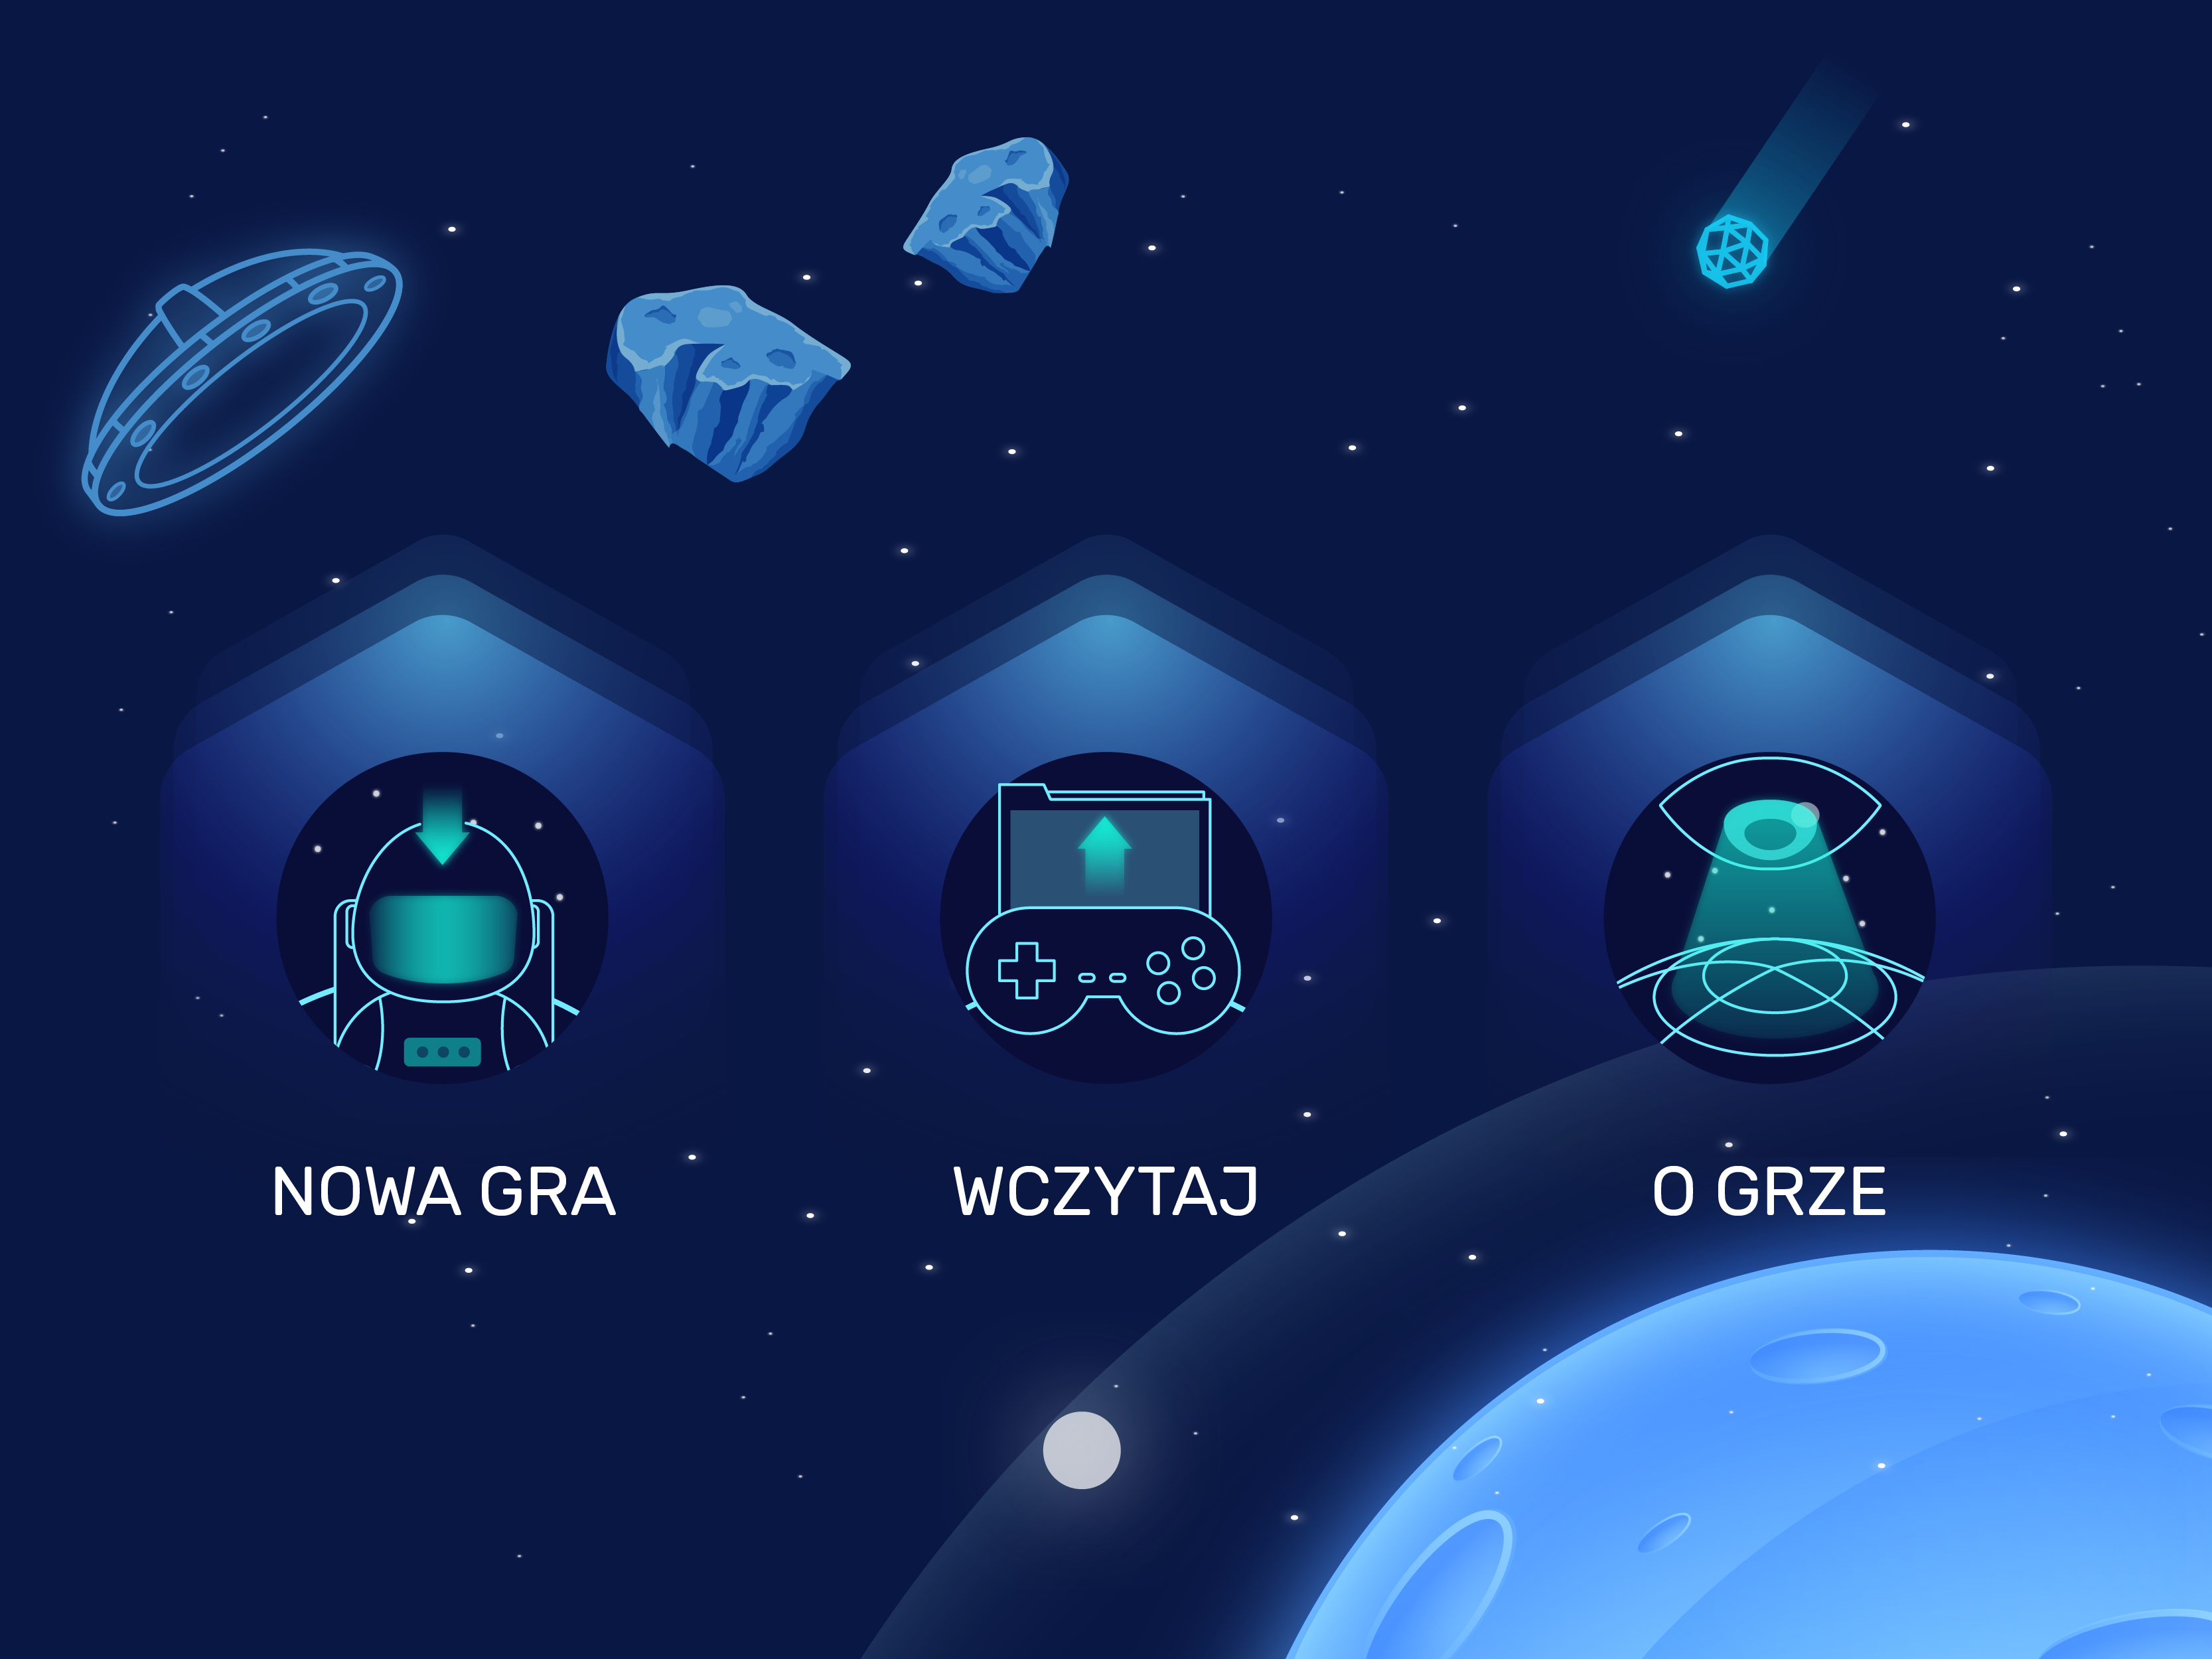
\includegraphics[width=1\textwidth]{img/ekran-start.png}
    \caption{Ekran startowy}
    \label{fig:start}
\end{figure}

\newpage

\paragraph{}Na rysunku \ref{fig:gracze}. możemy dostrzec ekran pozwalający nam na wprowadzenie nazw graczy i przejście do następnego kroku.
\begin{figure}[H]
    \centering
    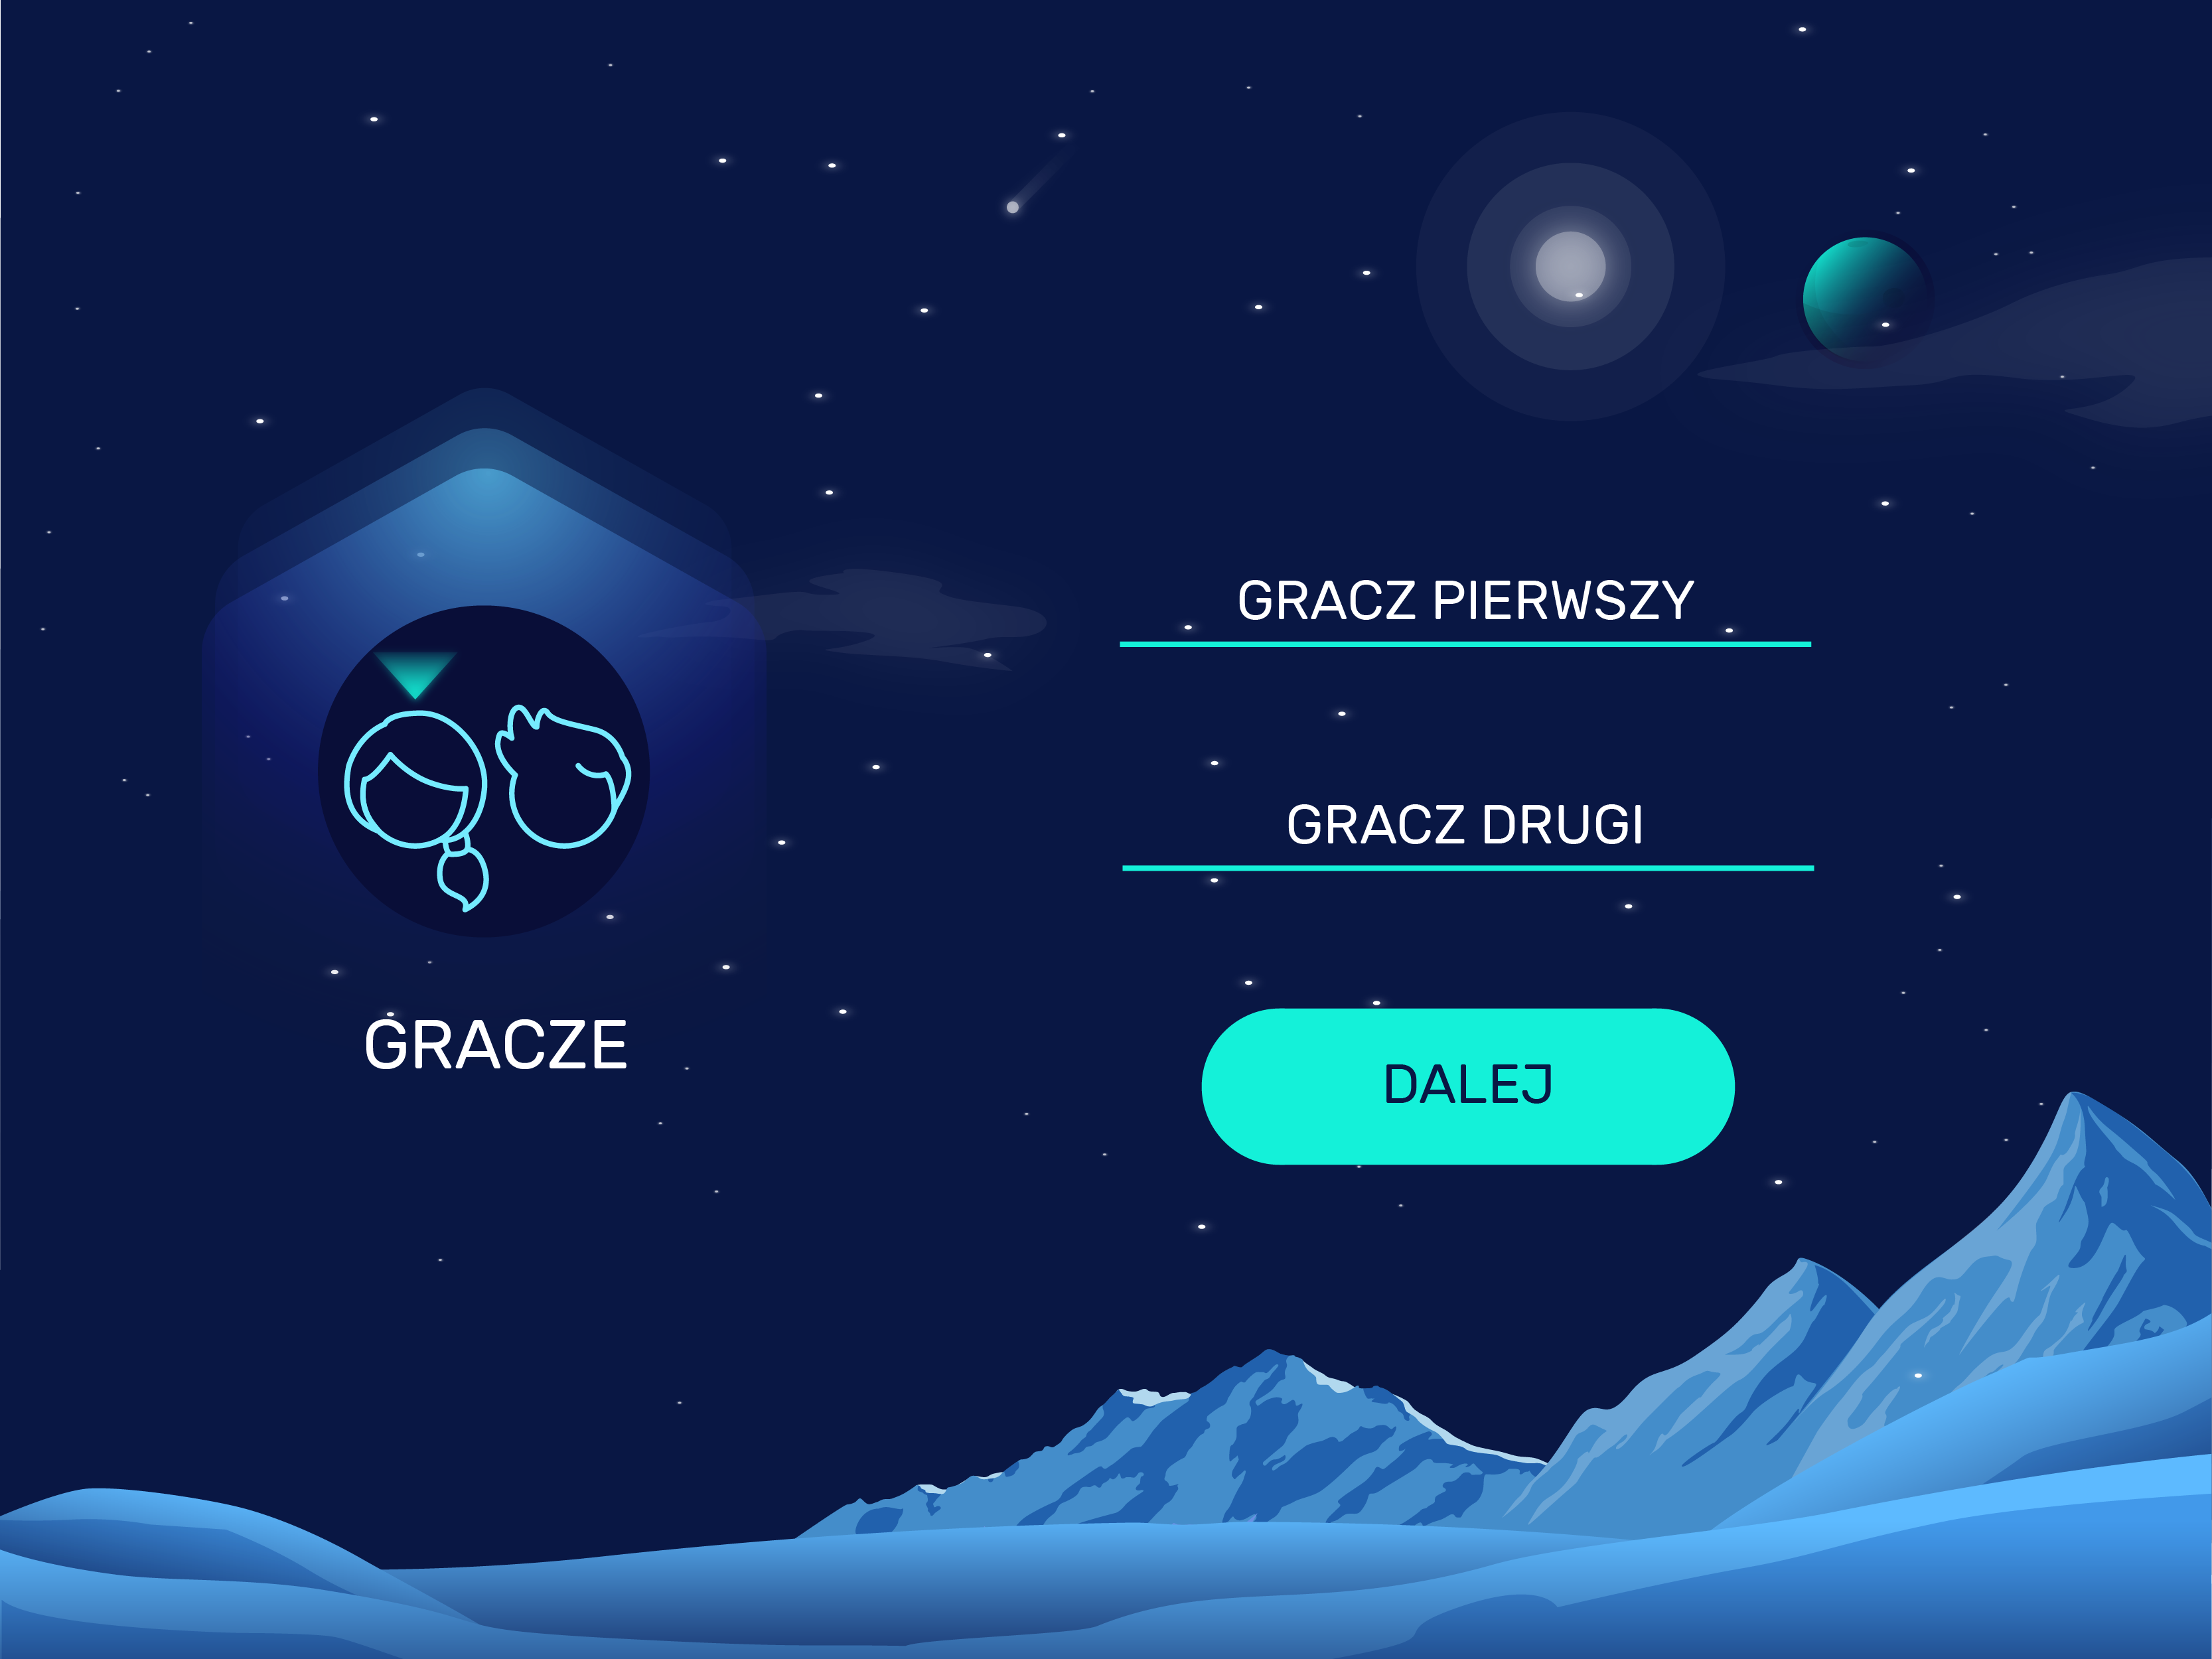
\includegraphics[width=1\textwidth]{img/ekran-gracze.png}
    \caption{Ekran wprowadzania imion graczy}
    \label{fig:gracze}
\end{figure}

\newpage

\paragraph{}Kolejna grafika (rys. \ref{fig:wczytaj}.) ukazuje nam ekran, przy pomocy którego możemy ręcznie wprowadzić ścieżkę do pliku w polu tekstowym. Ikona folderu przy końcu linii pozwala użytkownikowi otworzyć okno systemowe z wyborem pliku na dysku, co powinno ułatwić jego odnalezienie. Przycisk \textit{DALEJ} umożliwia przejście do następnego kroku.
\begin{figure}[H]
    \centering
    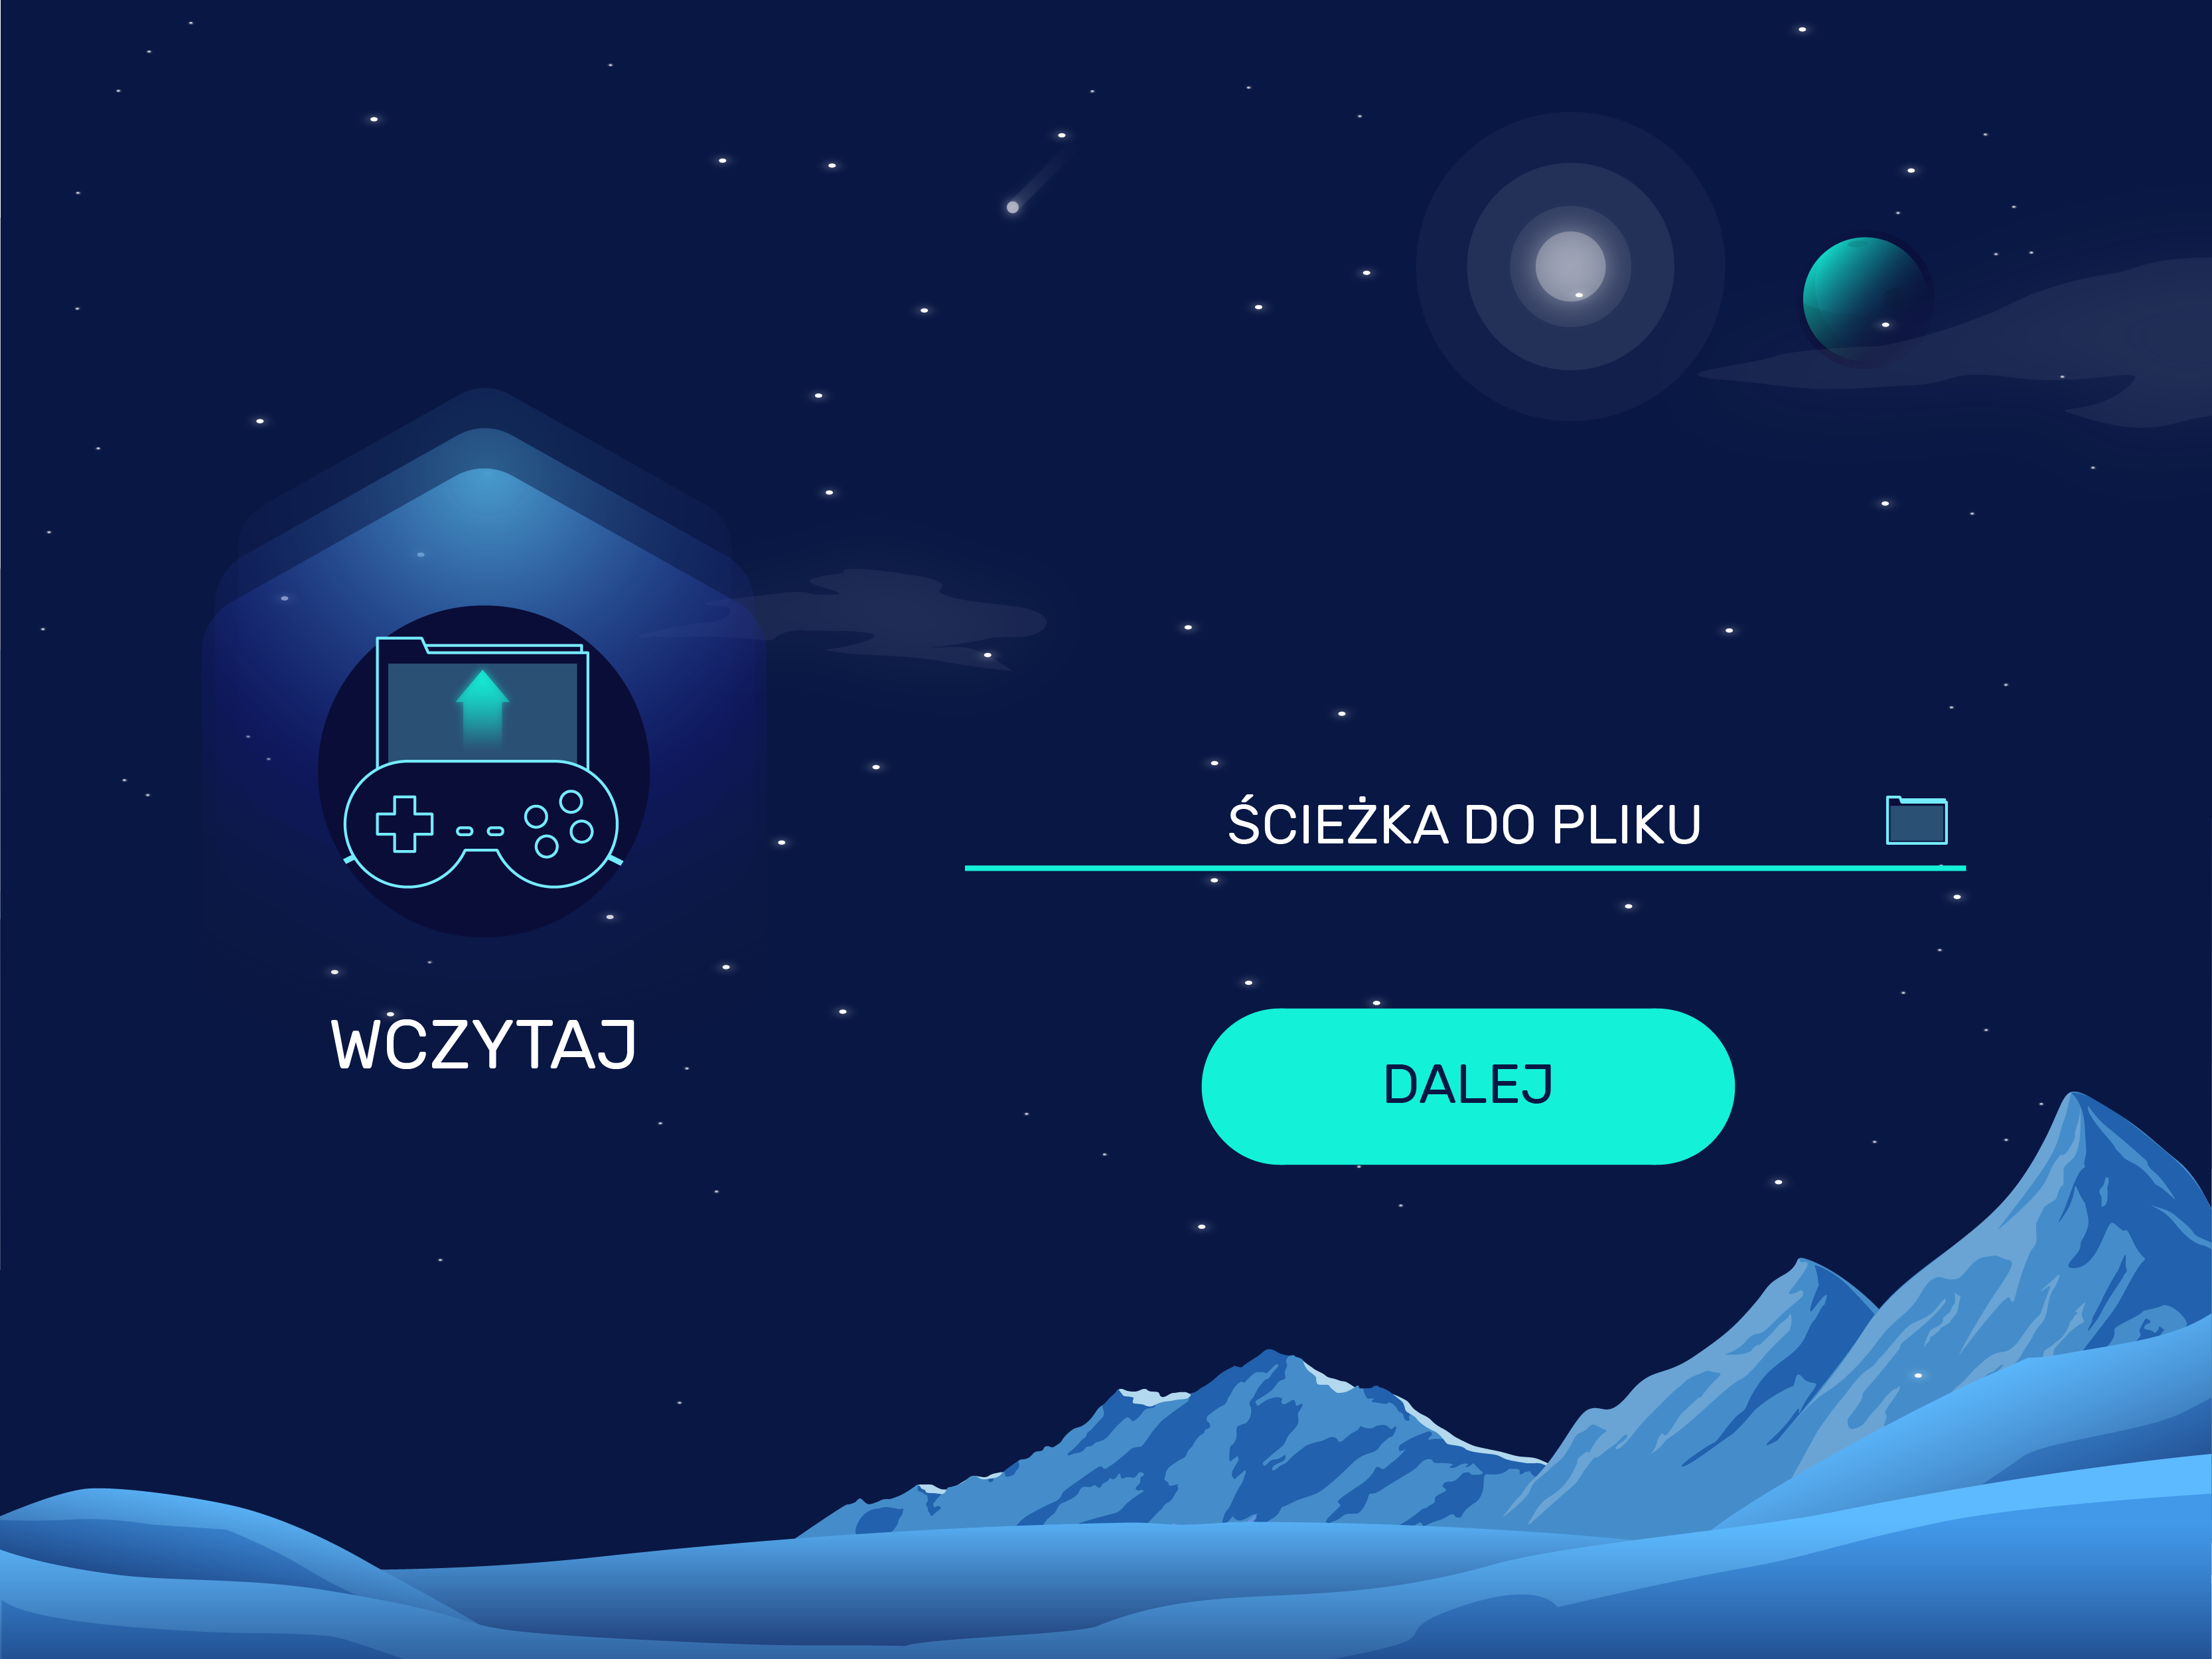
\includegraphics[width=1\textwidth]{img/ekran-wczytaj.png}
    \caption{Ekran wczytywania gry}
    \label{fig:wczytaj}
\end{figure}

\newpage

\paragraph{}Na ekranie przedstawionym na rysunku \ref{fig:o grze}. zostanie zamieszczona informacja o grze i instrukcja do niej. Istnieje możliwość powrotu do menu głównego przy pomocy przycisku \textit{WRÓĆ}.
\begin{figure}[H]
    \centering
    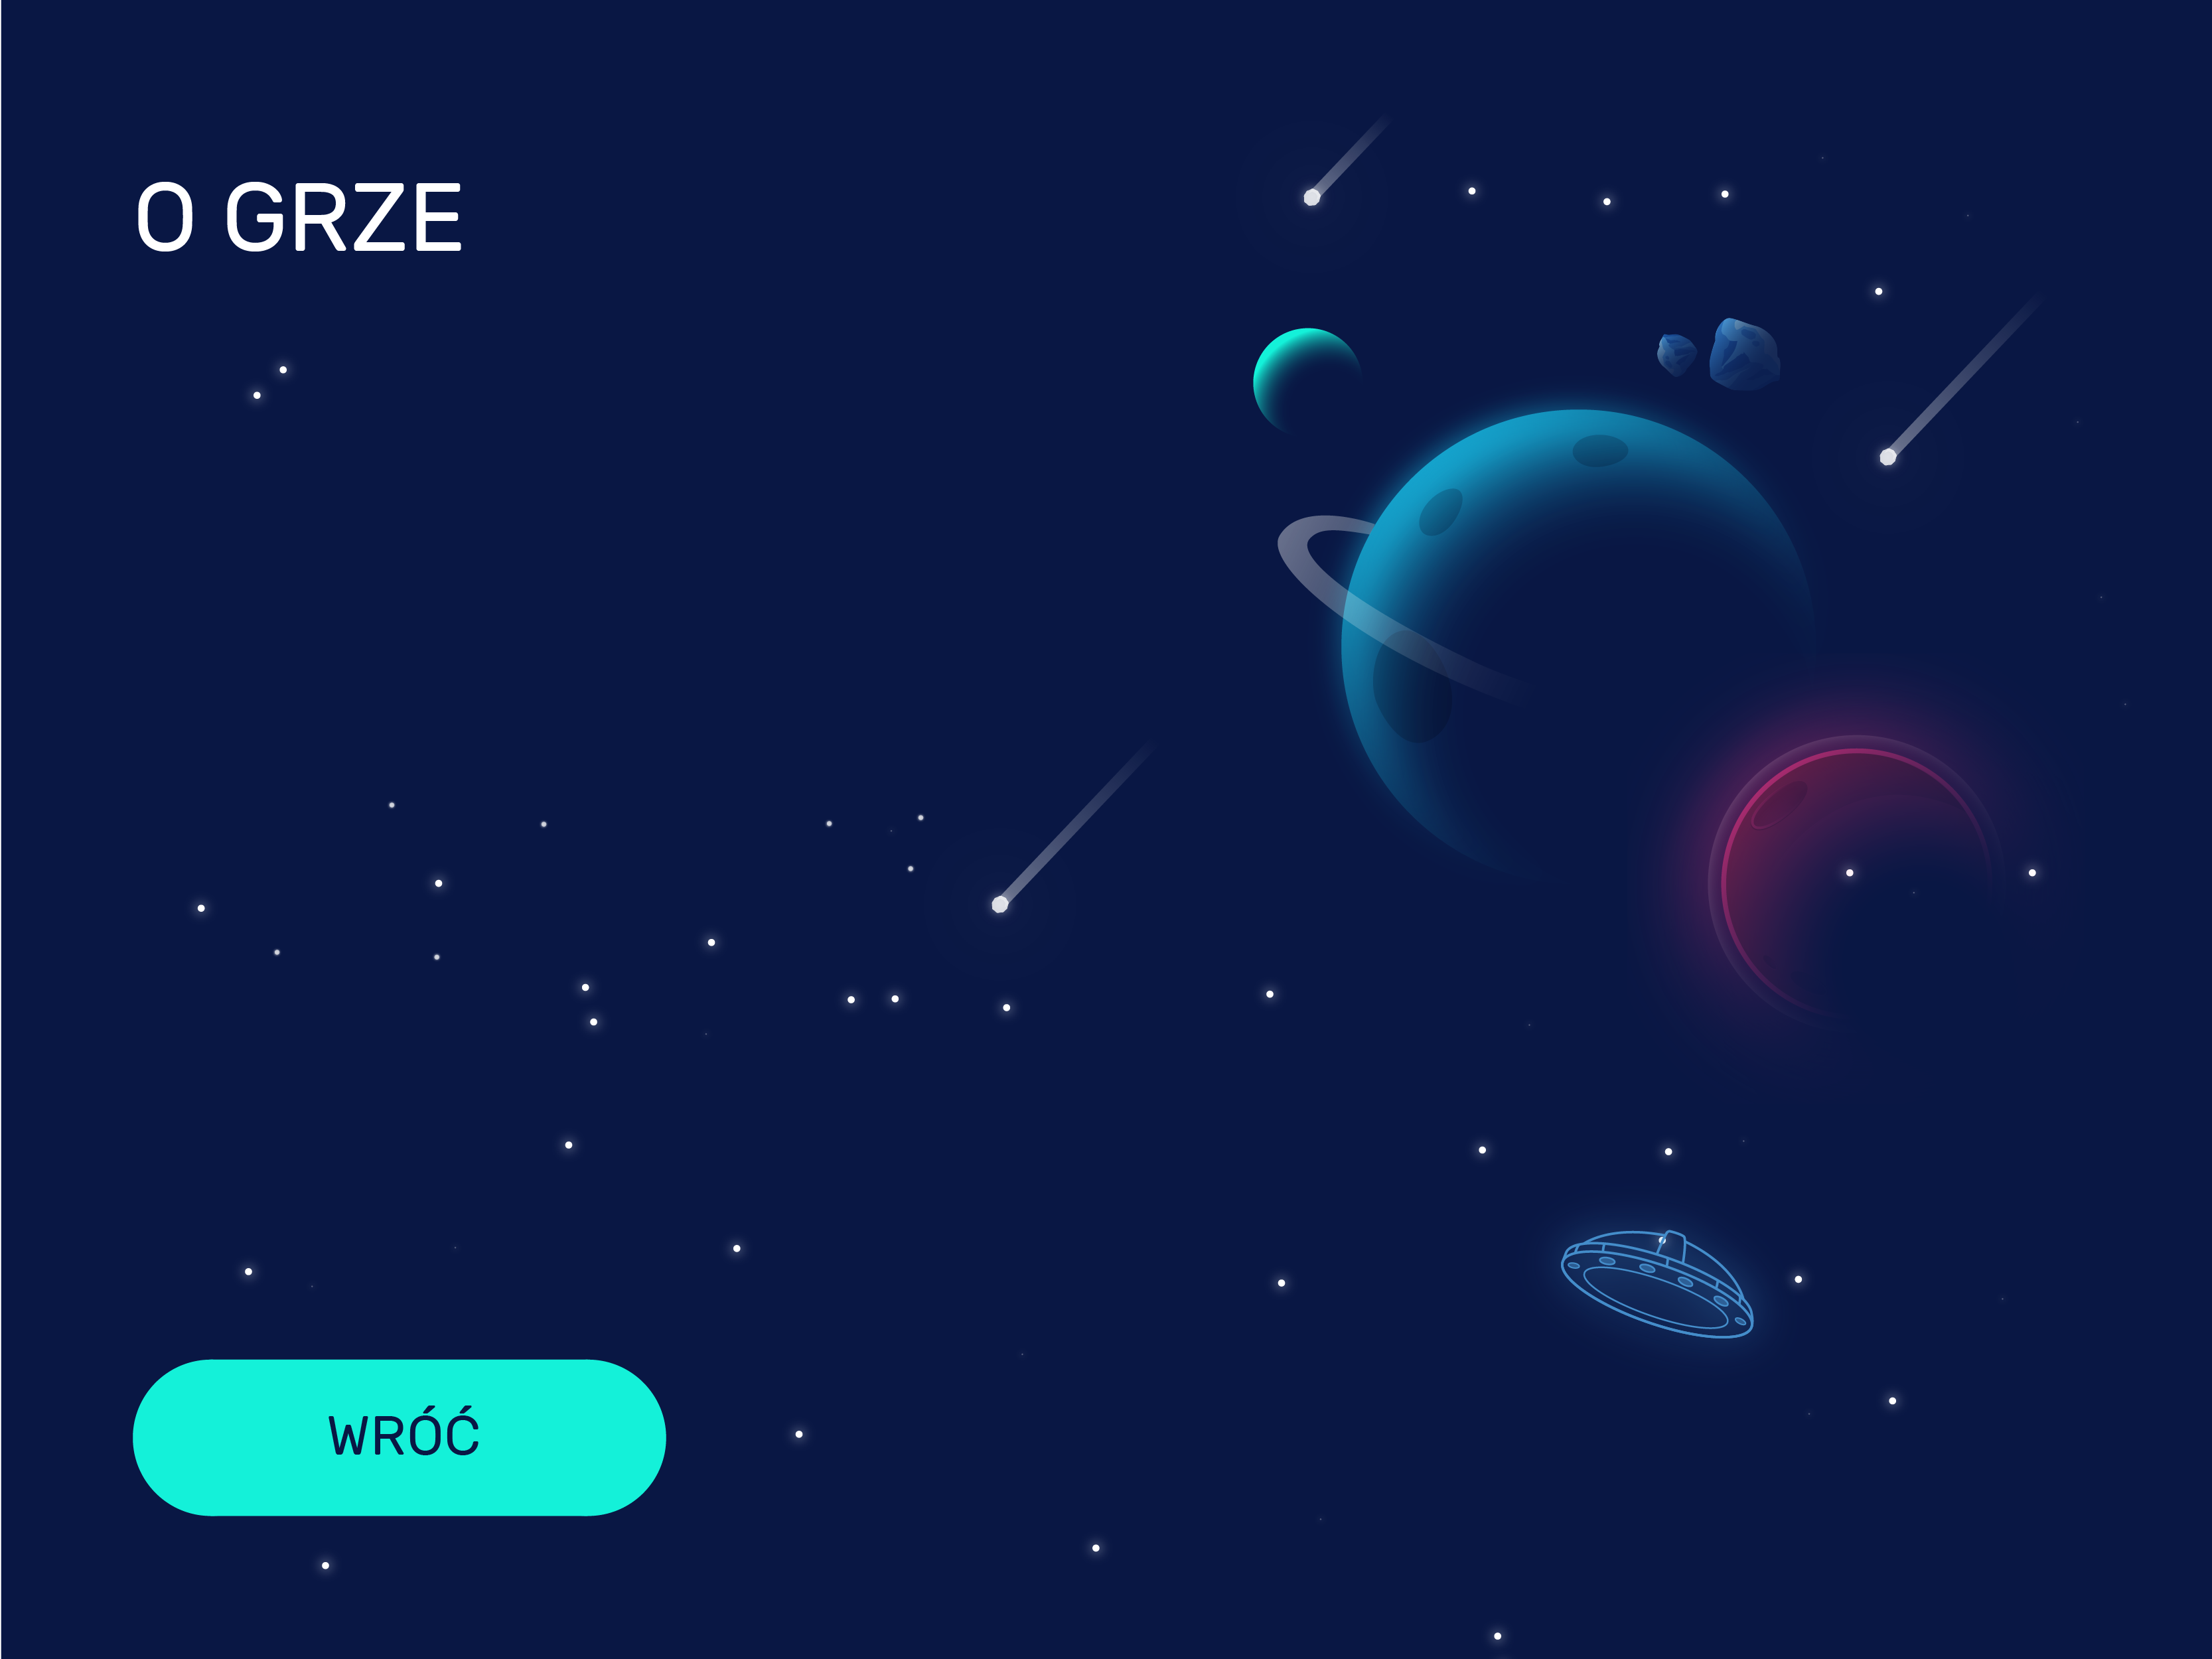
\includegraphics[width=1\textwidth]{img/ekran-o-grze.png}
    \caption{Ekran o grze}
    \label{fig:o grze}
\end{figure}

\newpage

\paragraph{}Rysunek \ref{fig:gra}. prezentuje:
\begin{itemize}
    \item planszę,
    \item spadające klocki (wrogów),
    \item statki,
    \item lasery,
    \item zegar czasu gry,
    \item liczniki punktów,
    \item licznik poziomów,
    \item imiona graczy,
    \item przyciski pozwalające na przerwanie gry i/lub zapisanie jej do pliku.
\end{itemize}
\begin{figure}[H]
    \centering
    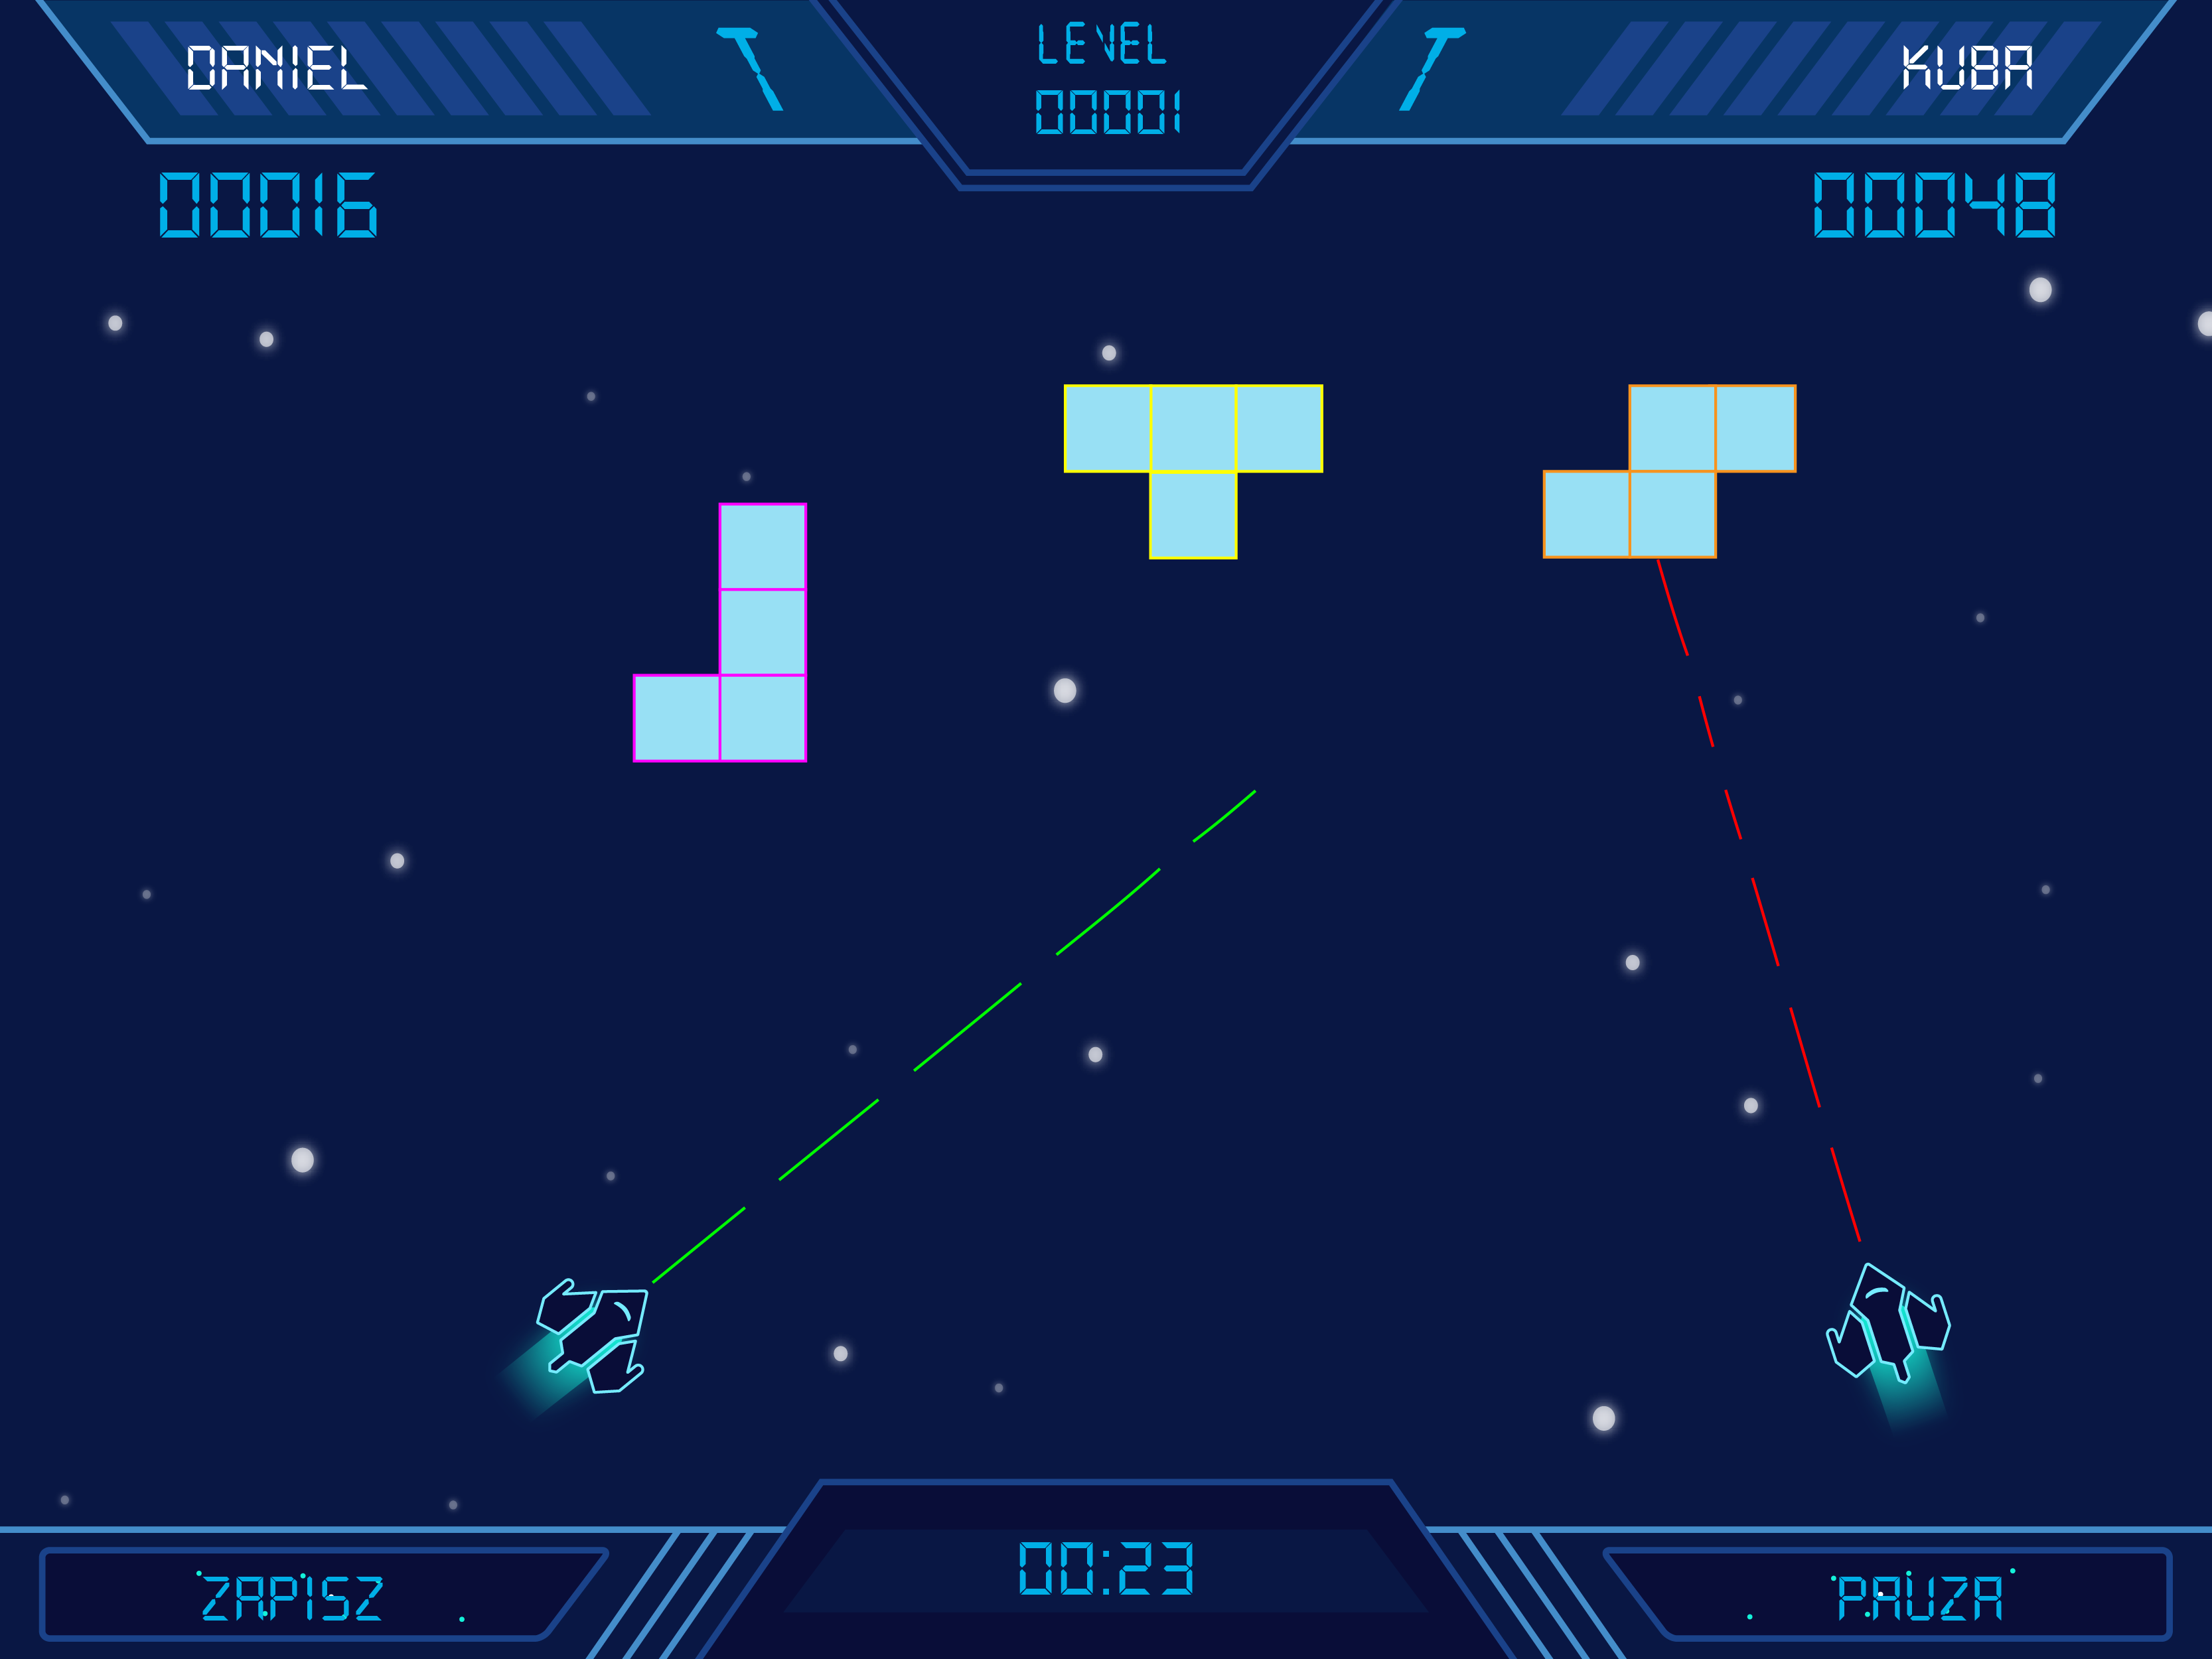
\includegraphics[width=1\textwidth]{img/ekran-gry.png}
    \caption{Ekran gry}
    \label{fig:gra}
\end{figure}

\newpage

\paragraph{}Na rysunku \ref{fig:pauza}. możemy zaobserwować przyciski \textit{WZNÓW, ZAPISZ, WYJDŹ,} których działanie dokładnie opisane jest w podrozdziale \ref{ss} pkt \ref{pauza}.
\begin{figure}[H]
    \centering
    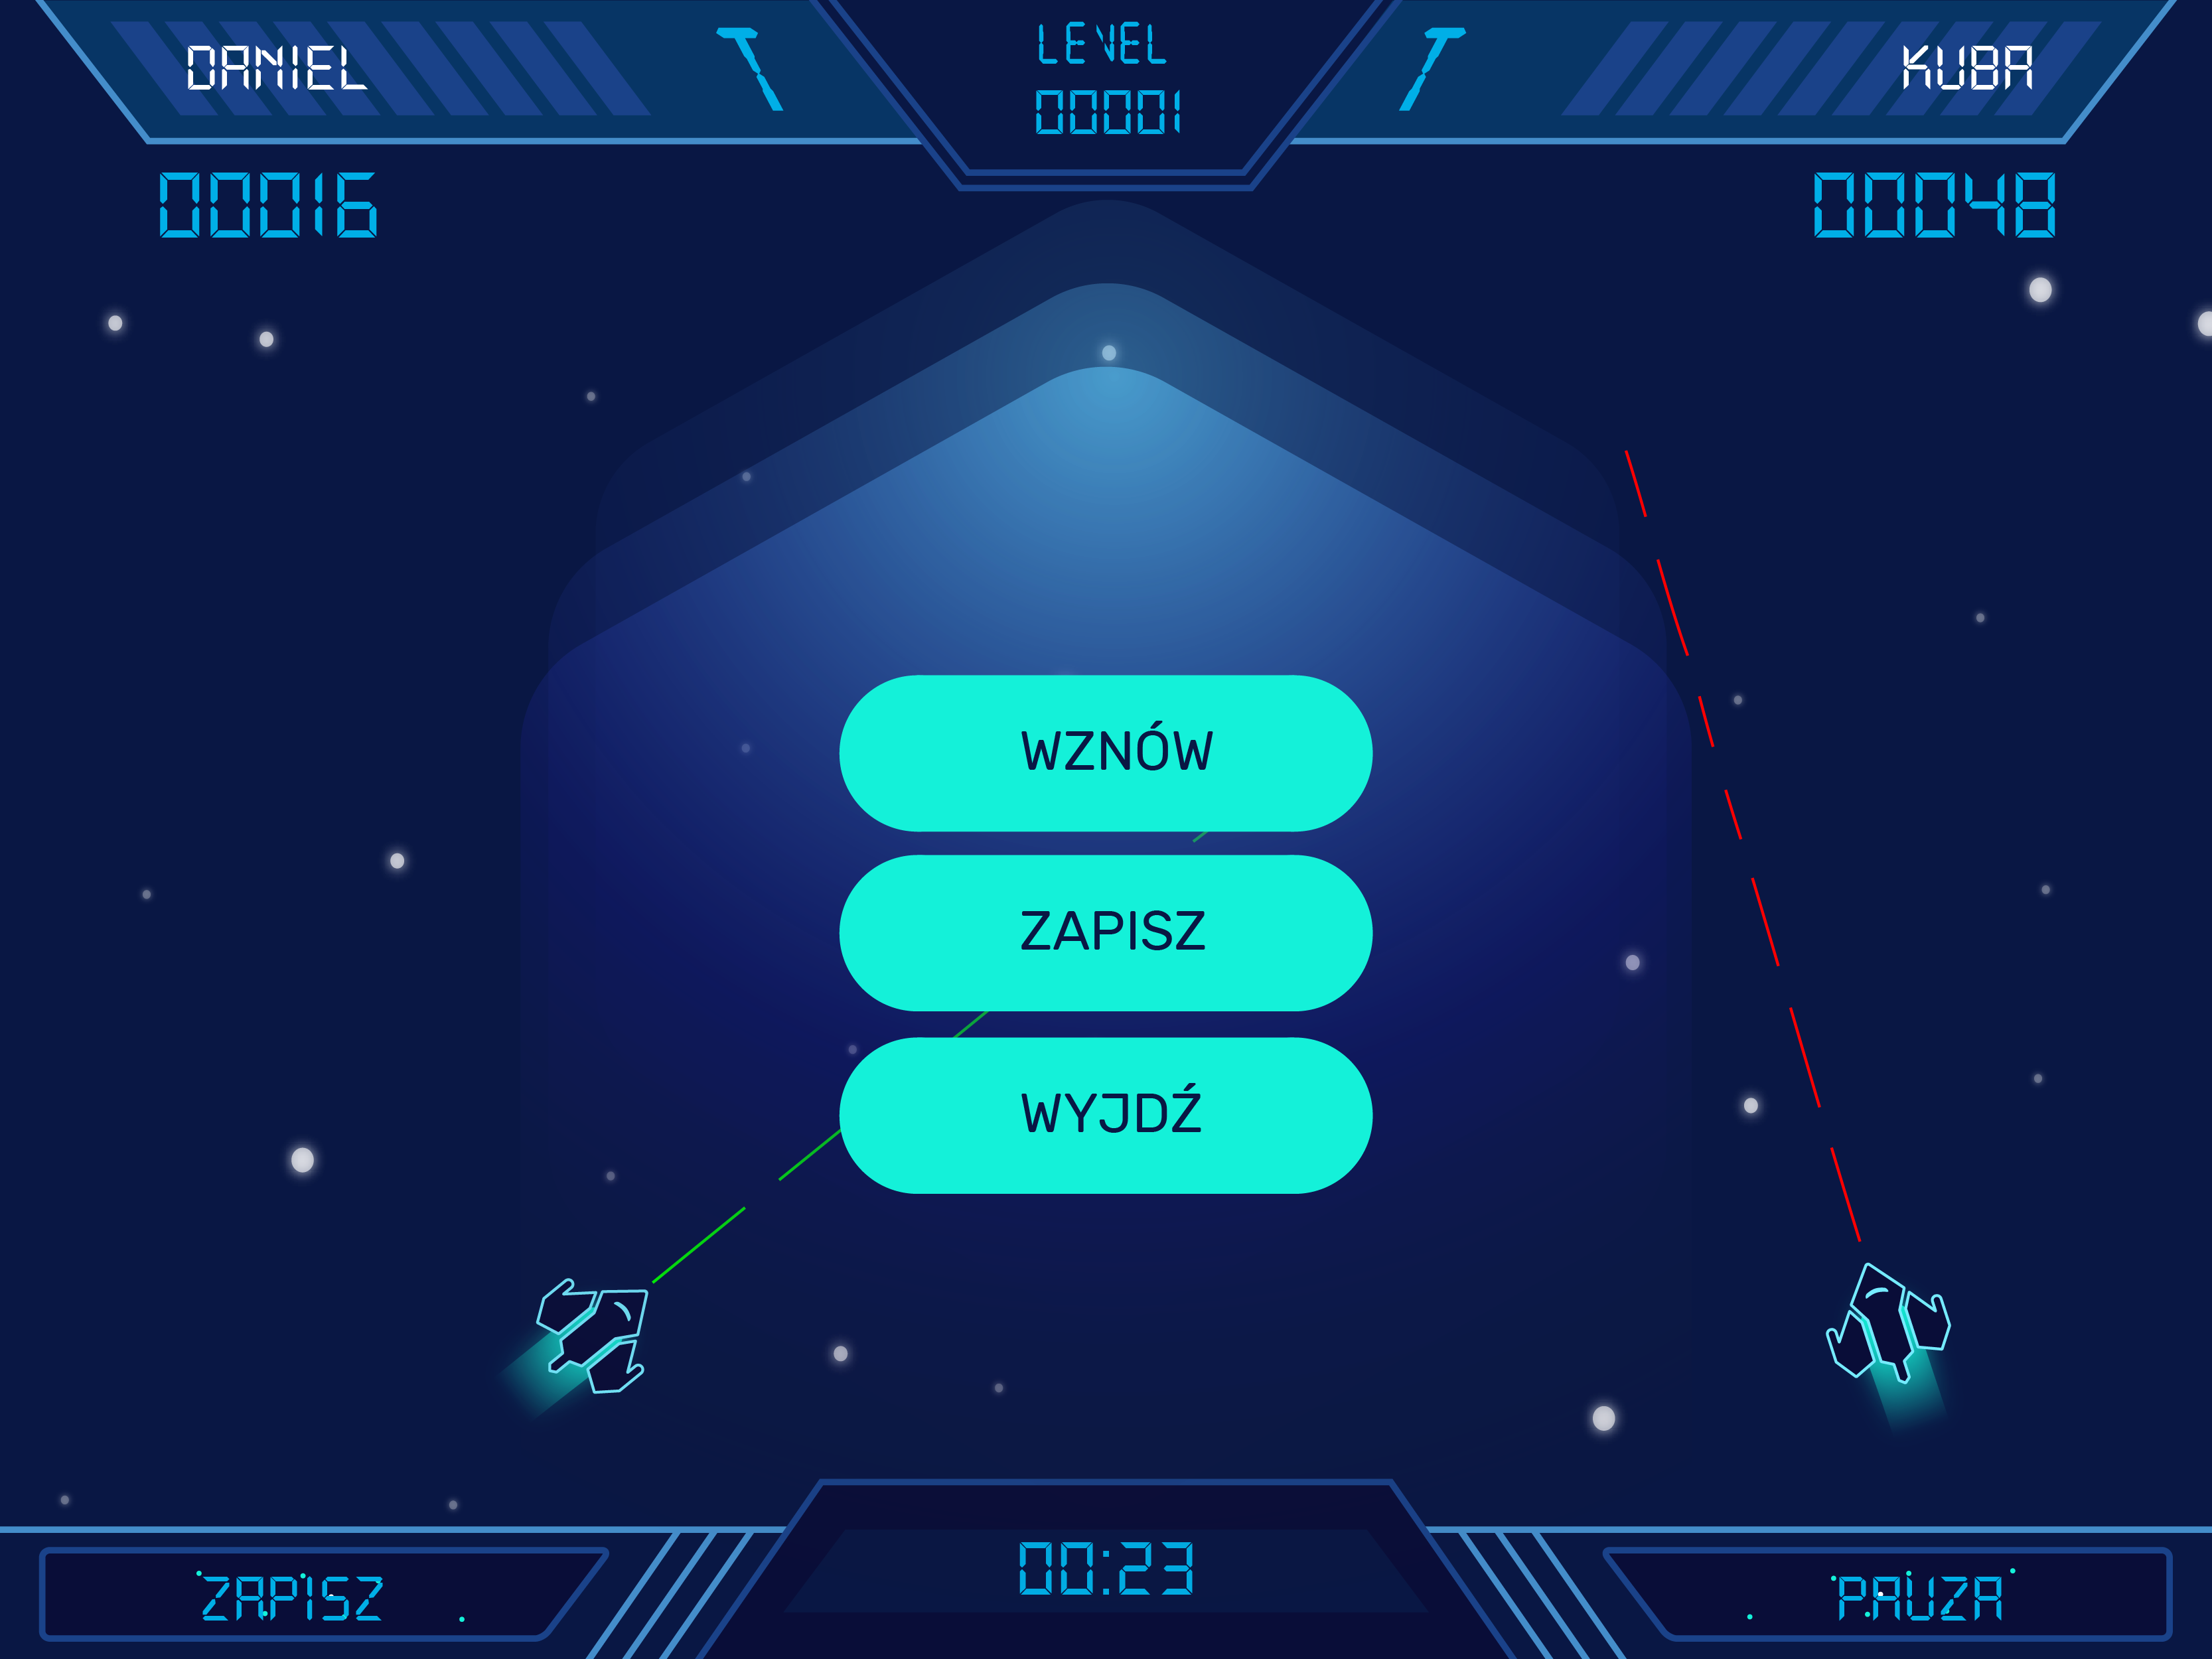
\includegraphics[width=1\textwidth]{img/ekran-pauza.png}
    \caption{Ekran zatrzymania gry}
    \label{fig:pauza}
\end{figure}

\newpage

\paragraph{}Rysunki \ref{fig:wygrana}. i \ref{fig:game over}. reprezentują ekrany końca gry.\\
Rysunek \ref{fig:wygrana}. zostanie wyświetlony, gdy w momencie ukończenia gry jeden z graczy ma większą liczbę punktów niż drugi. Liczba ta musi być dodatnia.\\
Rysunek \ref{fig:game over}. zostanie wyświetlony, gdy w momencie ukończenia gry obaj gracze będą mieli ujemną liczbę punktów lub dojdzie do remisu.
\begin{figure}[H]
    \centering
    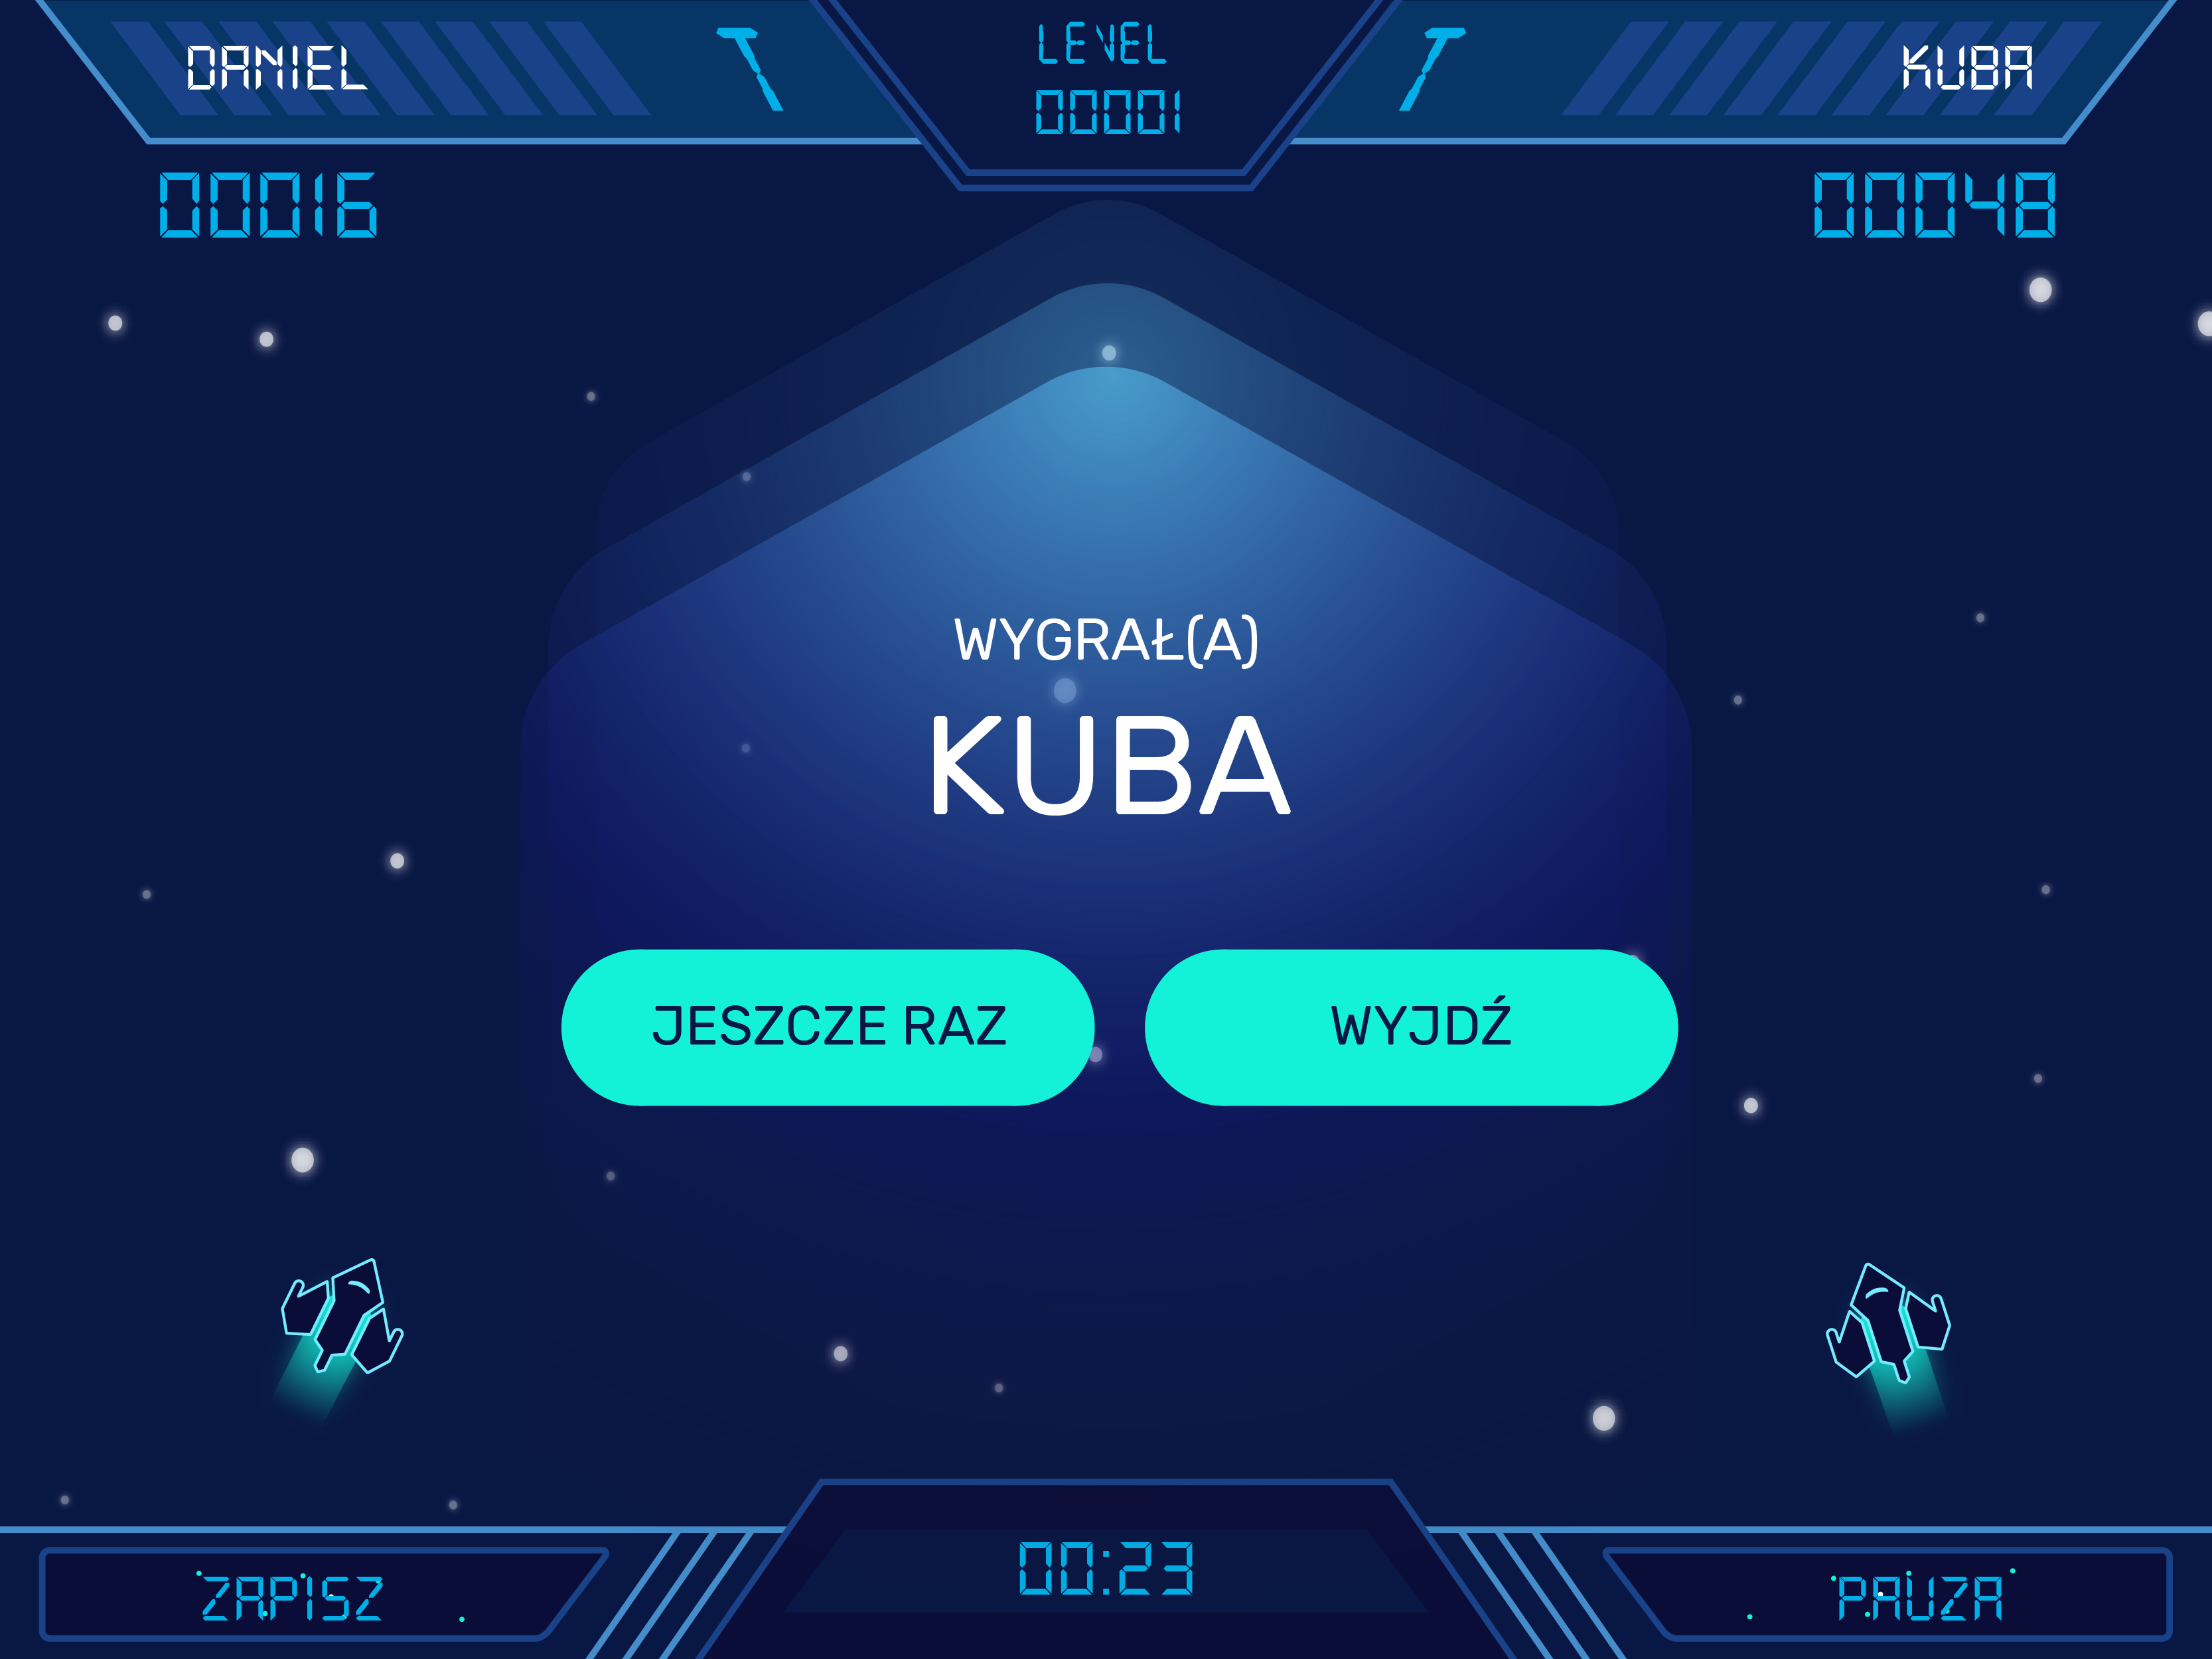
\includegraphics[width=1\textwidth]{img/ekran-wygrana.png}
    \caption{Ekran wygranej}
    \label{fig:wygrana}
\end{figure}
\begin{figure}[H]
    \centering
    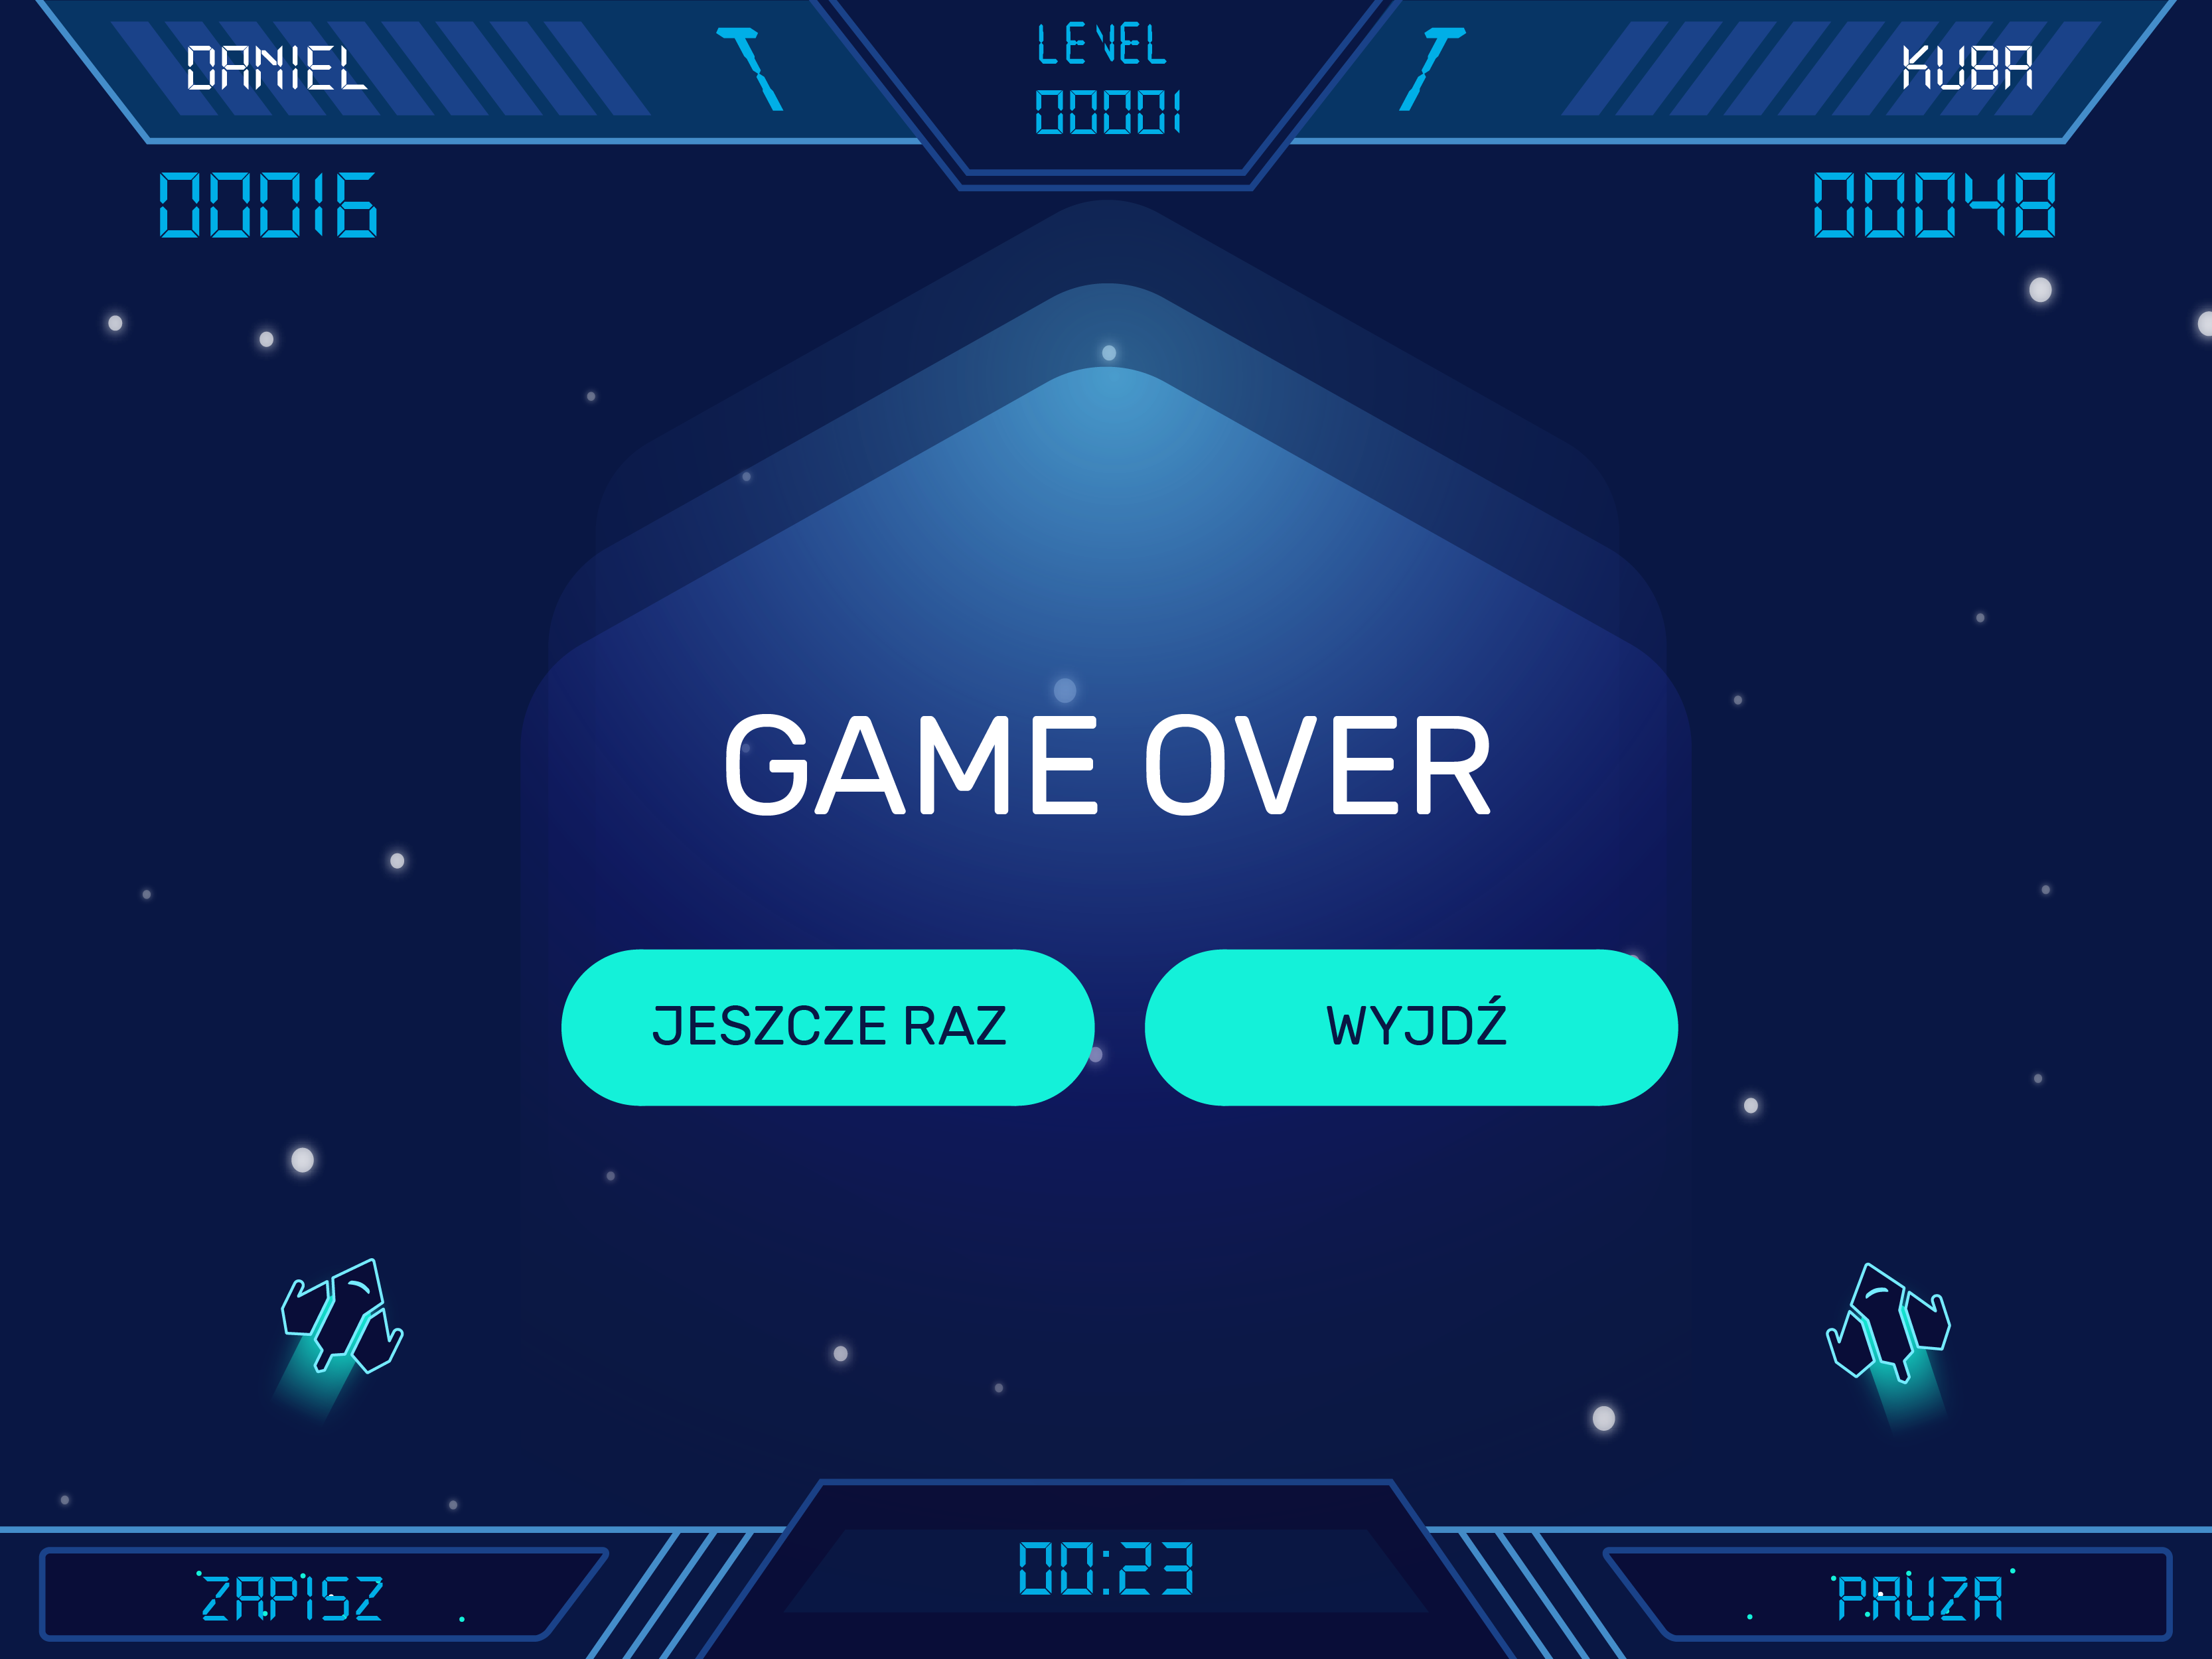
\includegraphics[width=1\textwidth]{img/ekran-game-over.png}
    \caption{Ekran przegranej}
    \label{fig:game over}
\end{figure}

\paragraph{}\textit{Pojedyncze elementy grafiki wektorowej i fonty użyte do przygotowania poglądowych rysunków pochodzą z otwartych źródeł. Licencje pozwalają na ich bezpłatne wykorzystanie (bez obowiązku podania autora) zarówno w projektach prywatnych jak i komercyjnych. Wszystkie powstałe do projektu wizualizacje są naszą autorską inwencją twórczą.}

\section{Testowanie}
\subsection{Ogólny przebieg testowania}
Do przetestowania kodu użyjemy narzędzi z biblioteki AssertJ. Natomiast GUI przetestujemy ręcznie podczas tworzenia aplikacji. Dodatkowo gotowy program przetestujemy sami, grając w niego oraz przekażemy go do testów znajomym.
\label{end}

\end{document}